%!TEX root = ../template.tex
%%%%%%%%%%%%%%%%%%%%%%%%%%%%%%%%%%%%%%%%%%%%%%%%%%%%%%%%%%%%%%%%%%%
%% chapter1.tex
%% NOVA thesis document file
%%
%% Chapter with introduction
%%%%%%%%%%%%%%%%%%%%%%%%%%%%%%%%%%%%%%%%%%%%%%%%%%%%%%%%%%%%%%%%%%%

\typeout{NT FILE chapter1.tex}

\chapter{Introduction}
\label{sec:objectives}

In the process of any given interaction, humans will naturally reveal a vast arrangement of signals independently from speech. Physical traits such as posture, gait or eye contact come under the social phenomenon known as non-verbal behaviour. Other examples of these cues commonly studied in the literature include facial expressions and tone of voice \cite{chanel_connecting_2015,carton_nonverbal_1999}, assuming a kind of social cue that's observable during a conventional human-human exchange when given deliberate attention. However, we should also take into account the changes that take place inside the body, being those not so easily perceived without way of technological intervention.

\section{Motivation}
\label{intro:matoivation}

Affective Computing and specifically the combination of physiological sensing and cognitive frameworks, has been an active field of study for over two decades \cite{picard_affective_2000}, securing prospects for developing emotionally-informed systems. A significant progression in this field can be conclusive of using state-of-the-art machine learning (and deep learning) methods to interpret large-scale datasets, achieving honourable breakthroughs in view of emotion recognition studies \cite{bota_review_2019}. Such systems tend to operate according to linguistic descriptors of universal emotions, a process known as the informational view \cite{boehner_how_2007}. From a communication standpoint, we recognise that these discrete representations become less meaningful when perceived in lack of contextual information. An emerging area of research considers the role of interactive systems for sharing physiological activity between users, enhancing connectedness by way of anatomical transparency \cite{lux_live_2018}. The resulting artefacts tend to utilise raw forms of data representation, disregarding emotional interpretation. Simultaneously, embodied sensor technology has been incorporated into creative practices, commonly as a means to capture emotional qualities of bodily gestures during performance, and then being able to transmit this information to a third-person perspective \cite{fdili_alaoui_seeing_2017}.

In addition, aesthetic representations have been incorporated into a wide range of user-centred technologies, observed by the broader vision of third-wave Human-Computer Interaction (HCI), through the comprehension that aesthetics are not bound to formal artistic creation but an essential function of sensorial engagement \cite{bodker2015third}. Building upon these trends, novel systems have been capable of capturing and mediating the emotional experiences that present themselves in everyday life \cite{schiphorst_designing_2020}.

We identify a motivation and methodology for using wearable sensors as an expressive resource for speechless dialogue, putting aesthetics at the forefront of interaction. Initialised from a thorough discussion on state-of-the-art technologies and established design principles regarding this topic, then applied to a novel approach alongside a selection of practical works to complement this. Given the preliminary proposition of non-representation, the intention is not to infer or classify emotion but rather to create new opportunities for rich gestural exchange, unconfined to the verbal domain. Embracing the right to express oneself from the within, taking the heart, lungs, muscles and motor activity as a basis for maintaining expressive speechless dialogue through the act of being present with the self, others and social environment.

\section{Core Research Questions}
\label{sec:research_questions}

This work focuses on three main research questions: (1) Why should embodied sensor technologies be used to mediate non-verbal dialogue? (2) What mediums are capable of producing emotionally meaningful representations of physiological signals, suitable for social intervention? And (3), by adopting methods from modern Machine Learning and New Media practices, how can aesthetics be incorporated into visuals, sound and haptic mechanisms to articulate and express emotional content? And how does this encourage user empowerment and penalisation for effective intervention? Each of these components are further detailed in the following segment.

% \begin{enumerate}
%     \item \textbf{Why} should embodied sensor technologies be used to mediate speechless dialogue?
%     \item \textbf{What} mediums are capable of producing emotionally meaningful representations of physiological signals, suitable for social intervention?
%     \item \textbf{How. } Adopting methods from modern Machine Learning and New Media practices, \textbf{how} can aesthetics be incorporated into visuals, sound and haptic mechanisms to articulate and express emotional content? And \textbf{how} do we encourage user empowerment and penalisation for effective intervention?

% \end{enumerate}

\begin{enumerate}
    \item \textbf{Why.} Given the layers of novelty and interdisciplinary nature of our work, weaving between the domains of data science, psychology, artistic performance and interaction design, we commit to delivering a comprehensive review of relevant research actions presented in the state-of-the-art, and validate our appropriation of such technologies and practices.

    \item \textbf{What.} Part of our research is also devoted to evaluating specific technologies that can be used. Starting from the common wearable sensing modalities, reviewing the interactive affordances of each, along with their corresponding feature extraction methods to retrieve emotionally relevant information. We evaluate methods for producing novel representations and the appropriate mediums for communicating this between users, whether that be through sound, visual or hardware-based interaction, in a way that balances aesthetic and informational qualities.

    \item \textbf{How.} By adopting user-centred design principles from third-wave HCI research, already demonstrating success in these areas, we aim to push more towards technical transparency, in that the user is really a part of the design process and consequentially feels a sense of authority over the system. This assumes a level of responsibility towards proactive sense-making, by way of parameter adjustment, personal contributions to datasets, and voluntary participation.
\end{enumerate}

\section{Collaborations and Affiliations}

The works presented have been realised as a result of the collaborations between academic, industry and cultural representatives. The following have sustained the research process in providing the financial, technical and human resources necessary to successfully carry out the user studies. The individual contributions derived from these collaborations will be explicitly noted where applicable throughout the thesis document.

% \begin{itemize}
    % \item \textbf{AffecTech, Personal Technologies for Affective Health}

        The PhD research was partly funded by the Innovative Training Network “Marie Curie Actions” supported by the H2020 People Programme (GA 722022) entitled \textbf{AffecTech}, incentivised towards developing personal health technologies for affective disorders, and bridges expertise from physiology, engineering and interaction design. This interdisciplinary network is responsible for spawning the underlying motivations of the thesis, maintained through various collaborative research activities.

    % \item \textbf{PLUX Wireless Biosignals S.A.}

        The majority of the PhD was supported under the employment of \textbf{PLUX Wireless Biosignals S.A.}, responsible for supplying the foundation of technical materials used in the research outputs, namely the BITalino R-IoT device, along with sensory peripherals that were manufactured and customised in-house. This collaboration was intrinsic to the adoption of the specific materials used to develop our practical works while more generally being symbolic to the use of low-cost solutions for designing sensor-based applications.

    % \item \textbf{Moving Digits, Augmented Dance for Engaged Audience}

        A significant portion of the research was achieved in partnership with the Creative Europe initiative, \textbf{Moving Digits: Augmented Dance for Engaged Audience}. The team were responsible for coordinating field research in the context of dance performance over the course of two years. The project received local support from Madeira Interactive Technologies Institute (M-ITI) and Sõltumatu Tantsu Lava (STL), responsible for hosting the workshops and research residencies that are detailed in Sections \ref{preliminary_actions:modi_ws1} and \ref{case_studies:modi_dis}. The research team was also in charge of acquiring participants with specialist skill criteria to take part in the studies, specifically referring to a group of professional artists working at the intersection of contemporary dance and technology.

    % \item \textbf{KTH Royal Institute of Technology}

        The division of Interaction Design at \textbf{KTH Royal Institute of Technology} was responsible for hosting a personal research secondment that resulted in the research actions contained in Sections \ref{cha:Preliminary_Actions_sens_act} and \ref{case_studies:soma_chi}, accompanied by authoring contributions to the thesis publications. While having direct contact with highly acclaimed figures in the Somaesthetic design community \cite{hook_designing_2018}, these collaborations were immensely influential in our adoption of such principles exemplified in contemporary interaction design.
% \end{itemize}

\section{Thesis Structure}
\label{sec:structure}

\begin{figure}[htbp]
	\centering
	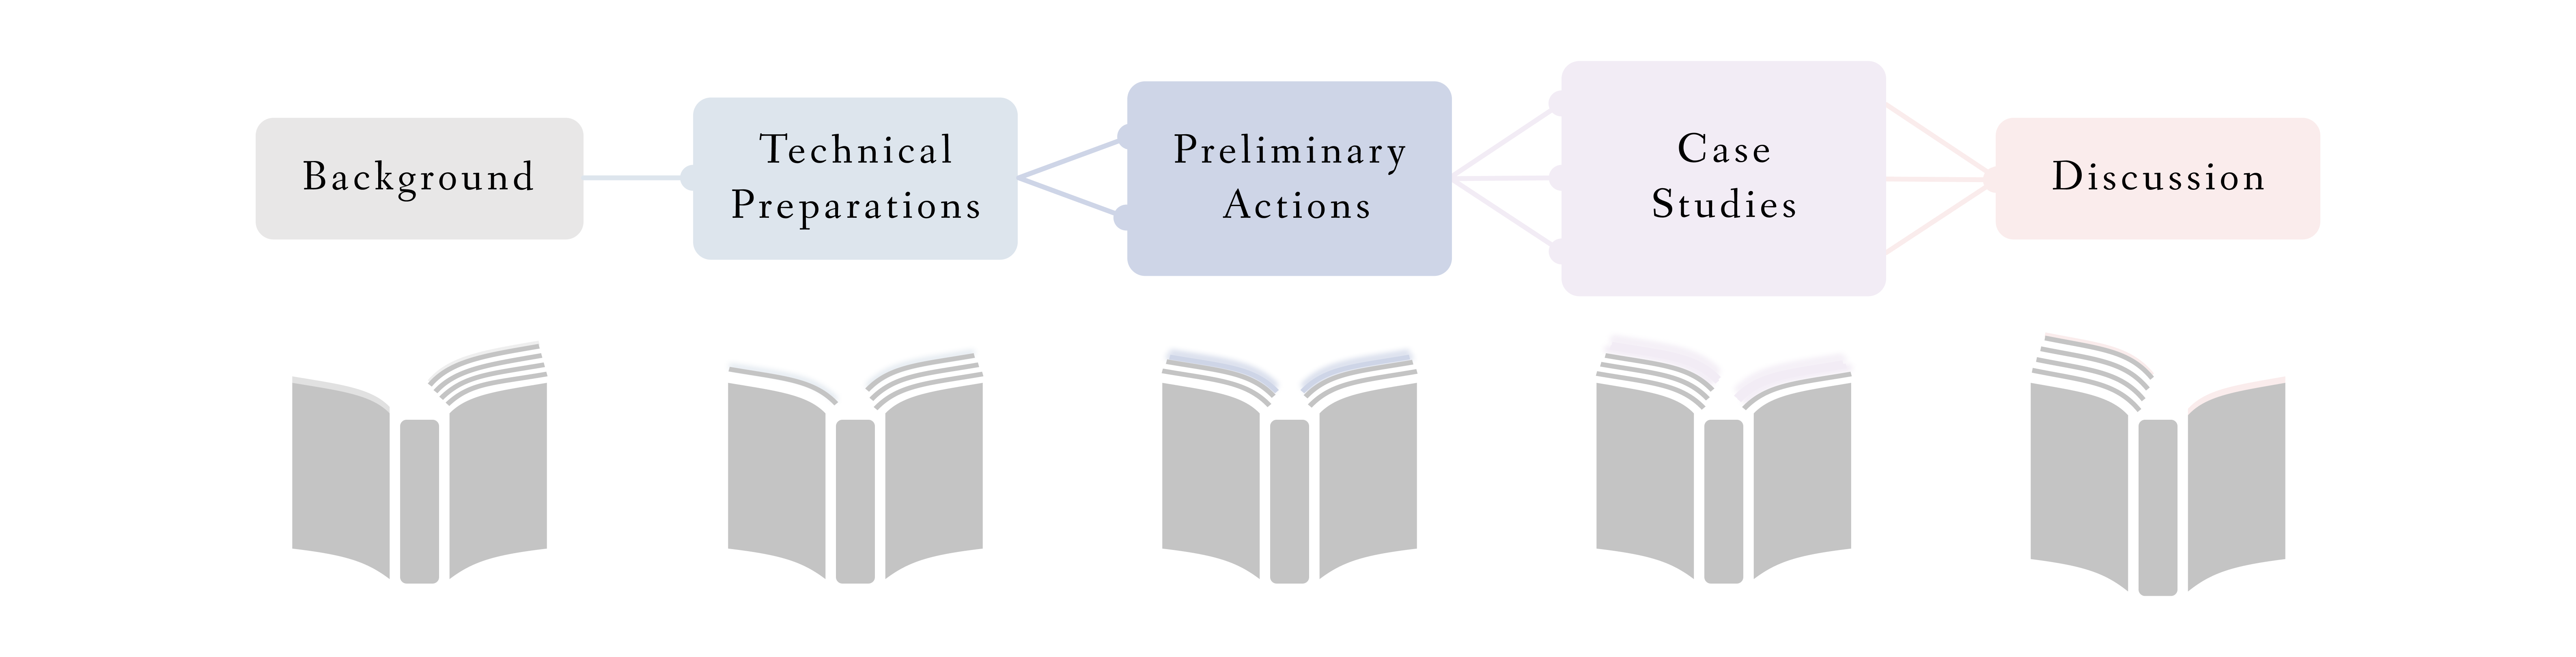
\includegraphics[width=1.0\textwidth]{Chapters/Figures/background/Sec1_Thesis_Structure}
	\caption{Thesis structure divided into five stages.}
	\label{fig:thesis_structure}
\vspace*{-20pt}
\end{figure}

\subsection*{Chapter 1: Introduction}
The current section briefly sets out the underlying motivation and raises the major research questions that run consistently throughout the thesis research.

\subsection*{Chapter 2: Theoretical and Technical Concepts}

Chapter \ref{cha:technical_concepts} provides a background to the technical and theoretical concepts that form the foundation of the thesis based upon four constructs: Non-verbal Communication; Physiological Sensors; The Aesthetic Domain; and Neural Networks. These constructs establish the major themes of the research and introduce conceptual bridges therein. From a technical standpoint, we provide a primer on the different physiological signals commonly used in the corresponding literature, noting their relevance and usability when applied in a given experimental context. We also take the opportunity to introduce some standard practices used in relevant research fields, such as Gesture Analysis, Social Signal Processing and the philosophical underpinning of Somaesthetics. Advancing from various topics grounded in computing and psychology research, we start to uncover a firm basis for aesthetic evaluation in the context of technological intervention as social-affective mediation.

\subsection*{Chapter 3: Literature Review}

In Chapter \ref{cha:lit_review}, we comment on some relevant literature covering the following key topics of interest, first looking at established research fields, namely, Affective Computing, Social Signal Processing, Interactive Machine Learning, Somaesthetic Design, and Non-Representational Theory. Then, to cover the broad domains of biosignals in creative practice, the appropriation of wearable sensors in creative practice and performance context, the social impact of sharing physiological activity and recognised methods for emotional representation are reviewed. Following an overview of a diverse range of topics and research outcomes, we try to draw out a conceptual narrative, justifying the intersection of these topics and identifying core design principles to be adopted into the research actions that follow, as described throughout the subsequent chapters.

\subsection*{Chapter 4: Technical Preparations}

In Chapter \ref{cha:technical_contributions}, we will introduce and examine a set of hardware and software tools developed within the duration of the PhD, and adopted to augment collaborative sensor-based interactions. This will include the design of specialised wearable devices for physiological data sensing in the wild, temperaments for latency estimation, and systems for processing and preparing sensor data for various interactive environments. An underlying aim here is to utilise web-based data transmission protocols to deploy interactive systems in a portable and spontaneous fashion, establishing a basis for studies to take place ``in the wild''.

\subsection*{Chapter 5: Preliminary Actions}

Our Preliminary Actions (Chapter \ref{cha:Preliminary_Actions}) are initiated with an individualistic exploration of input-output mediums for physiological representation, forming a broad foundation of aesthetic affordances when testing with our own bodies. Transitioning from an introspective experience, we prepare engagements with a selection of specialist user groups deemed suitable for providing new insights in a series of workshops comprised of focus group, data collection, ideation and evaluation stages.

\subsection*{Chapter 6: Major Case Studies}

Following these research actions, we present a collection of case studies that are realised using the knowledge organised from the prior research actions. In Chapter \ref{cha:case_studies} we will present a set of experimental systems developed during the PhD, each intended to establish a theoretical framework for designing systems for emotional exchange. Given this experimental methodology, a matured research space should provoke and sustain discussions around the socio-political implications of technological interventions and appropriation in preparation to be deployed in out-of-lab environments, eventually gearing towards pervasive engagement.

\subsection*{Chapter 7: Results and Discussion}

Finally, we can reflect on a multi-layered research process (Figure \ref{fig:thesis_structure}) and consolidate the overall outcomes rooted in the essential research appeal of the thesis. These are ultimately formulated as aesthetic considerations when designing for sensation, representation and communication in the context of sensory intervention. In Chapter \ref{cha:conclusion}, we open up to some of the major limitations present in our work, disclosing the additional paths for investigation, and closing the thesis with a call for future work in the push towards aesthetic engagement with communication technologies.

% \printbibliography[heading=subbibliography, segment=\therefsegment, title={\bibname\ for chapter~\thechapter}]
